\documentclass[11pt,letterpaper]{article}
\usepackage[margin=0.78in,headheight=14pt]{geometry}
\usepackage[T1]{fontenc}
\usepackage{lmodern,microtype}
\usepackage{amsmath,amssymb,booktabs,array,enumitem,xcolor,fancyhdr}
\usepackage{tikz}
\usetikzlibrary{shapes.geometric}
\usepackage[hidelinks]{hyperref}
\definecolor{ink}{HTML}{16344A}
\definecolor{muted}{HTML}{52616D}
\definecolor{leftboundary}{HTML}{0072B2}
\definecolor{rightboundary}{HTML}{D55E00}
\definecolor{logicaledge}{HTML}{8B4AA5}
\pagestyle{fancy}
\fancyhf{}
\fancyhead[L]{\small\sffamily\color{muted}SciCode 2 \enspace / \enspace Computational research challenge}
\fancyhead[R]{\small\sffamily\color{muted}Problem statement}
\fancyfoot[C]{\small\thepage}
\renewcommand{\headrulewidth}{0.3pt}
\setlength{\parindent}{0pt}
\setlength{\parskip}{0.55em}
\setlist[enumerate]{leftmargin=1.5em,itemsep=0.4em,topsep=0.25em}
\setlist[itemize]{leftmargin=1.4em,itemsep=0.3em,topsep=0.25em}
\newcommand{\sect}[1]{\vspace{0.55em}{\large\sffamily\bfseries\color{ink}#1}\par\vspace{0.15em}}
\newcommand{\F}{\mathbb F_2}
\newcommand{\Prob}{\mathbb P}
\newcommand{\ind}{\mathbf 1}
\newcommand{\loss}{P_{\mathrm{fail}}}
\begin{document}
\thispagestyle{fancy}
{\LARGE\sffamily\bfseries\color{ink}Decoding with Incomplete Local Witnesses\par}
\vspace{0.25em}
{\large\sffamily A two-parameter decoding phase diagram on a honeycomb lattice\par}

\sect{1. Scientific objective}
A parity measurement reveals whether an odd number of errors meet at a vertex,
but loses information about errors that cancel in pairs. Consider an additional
local measurement that can witness multiple incident errors, with an adjustable
probability of missing an eligible event. How does this information change the
ability to recover a logical bit as the lattice grows?

Develop, implement, and validate a computational approach to this question.
Your principal result must be a two-dimensional decoding phase diagram over
\[
             0\le p\le 1,\qquad 0\le q\le1,
\]
that identifies decodable and non-decodable regions and estimates or constrains
the transition boundary between them. Here $p$ controls physical errors and $q$
controls the availability of the local witness. Both are continuous parameters;
the aim is to understand the organization of the entire stated parameter domain.
Do not assume that the transition boundary is a single-valued function of $q$.

The phase diagram should explain how the prospect of reliable logical recovery
changes with $p$ and $q$ as the lattice grows. Support it with quantitative
finite-size evidence and uncertainty. The geometry, observation model, and
logical success criterion are specified below. You must choose and justify the
computational approach, approximations, and numerical evidence needed to reach
the scientific conclusion.

\sect{2. The stochastic experiment}
Let $G_L=(V_L,E_L)$ be the finite honeycomb patch defined on page~\pageref{geometry},
and let $D_L\subset V_L$ be its detector vertices. A trial consists of independent
binary errors on the retained edges:
\[
 x_e\sim\operatorname{Bernoulli}(p),\qquad e\in E_L.
\]
For each detector $v$, define its incident error count and observed parity by
\[
 n_v(x)=\sum_{e\ni v}x_e,\qquad s_v=n_v(x)\bmod2.
\]
The additional binary observation, called a \emph{herald}, is
\[
 h_v=\ind\{n_v(x)\ge2\}\,b_v,
 \qquad b_v\sim\operatorname{Bernoulli}(q).
\]
The $b_v$ are mutually independent and independent of all edge errors. Thus the
heralds are independent \emph{conditional on $x$}; their unconditional
correlations are part of the problem. Syndrome measurements are exact. There
are no false-positive heralds, additional readout errors, or repeated rounds.

A decoder receives only $(G_L,p,q,s,h)$, including the zero entries of $h$.
It has no access to $x$, $n_v$, $b_v$, error pairings, or microscopic histories.
No measurements are made at $V_L\setminus D_L$. A herald is a vertex
observation; it does not identify an erased or erroneous edge. This is a
stipulated classical noise-and-observation model; no microscopic fusion model
is required.

\newpage
\sect{3. Exact lattice and logical observable}\label{geometry}
The integer $L\ge2$ specifies the number of hexagon columns and rows, not the
code distance. Figure~\ref{fig:lattice} illustrates the construction below.
Use integer coordinates $(X,Y)$ and plotting coordinates $(X/2,\sqrt3Y/2)$.

\begin{center}
% BEGIN GENERATED LATTICE FIGURE
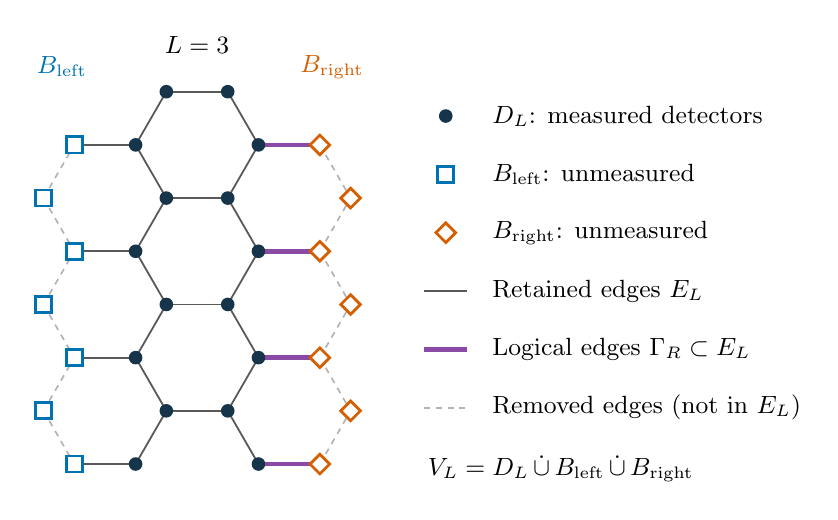
\begin{tikzpicture}[x=0.78cm,y=0.78cm,font=\small,
  kept/.style={draw=black!65,line width=0.65pt},
  removed/.style={draw=black!30,line width=0.6pt,dash pattern=on 2.2pt off 2pt},
  logical/.style={draw=logicaledge,line width=1.65pt},
  detector/.style={circle,fill=ink,draw=ink,inner sep=0pt,minimum size=4.5pt},
  leftv/.style={rectangle,fill=white,draw=leftboundary,line width=1pt,inner sep=0pt,minimum size=5.8pt},
  rightv/.style={diamond,aspect=1,fill=white,draw=rightboundary,line width=1pt,inner sep=0pt,minimum size=7.5pt}]
\draw[removed] (-1.000000,0.000000) -- (-0.500000,-0.866025);
\draw[removed] (-1.000000,0.000000) -- (-0.500000,0.866025);
\draw[removed] (-1.000000,1.732051) -- (-0.500000,0.866025);
\draw[removed] (-1.000000,1.732051) -- (-0.500000,2.598076);
\draw[removed] (-1.000000,3.464102) -- (-0.500000,2.598076);
\draw[removed] (-1.000000,3.464102) -- (-0.500000,4.330127);
\draw[removed] (3.500000,-0.866025) -- (4.000000,0.000000);
\draw[removed] (3.500000,0.866025) -- (4.000000,0.000000);
\draw[removed] (3.500000,0.866025) -- (4.000000,1.732051);
\draw[removed] (3.500000,2.598076) -- (4.000000,1.732051);
\draw[removed] (3.500000,2.598076) -- (4.000000,3.464102);
\draw[removed] (3.500000,4.330127) -- (4.000000,3.464102);
\draw[kept] (-0.500000,-0.866025) -- (0.500000,-0.866025);
\draw[kept] (-0.500000,0.866025) -- (0.500000,0.866025);
\draw[kept] (-0.500000,2.598076) -- (0.500000,2.598076);
\draw[kept] (-0.500000,4.330127) -- (0.500000,4.330127);
\draw[kept] (0.500000,-0.866025) -- (1.000000,0.000000);
\draw[kept] (0.500000,0.866025) -- (1.000000,0.000000);
\draw[kept] (0.500000,0.866025) -- (1.000000,1.732051);
\draw[kept] (0.500000,2.598076) -- (1.000000,1.732051);
\draw[kept] (0.500000,2.598076) -- (1.000000,3.464102);
\draw[kept] (0.500000,4.330127) -- (1.000000,3.464102);
\draw[kept] (0.500000,4.330127) -- (1.000000,5.196152);
\draw[kept] (1.000000,0.000000) -- (2.000000,0.000000);
\draw[kept] (1.000000,1.732051) -- (2.000000,1.732051);
\draw[kept] (1.000000,3.464102) -- (2.000000,3.464102);
\draw[kept] (1.000000,5.196152) -- (2.000000,5.196152);
\draw[kept] (2.000000,0.000000) -- (2.500000,-0.866025);
\draw[kept] (2.000000,0.000000) -- (2.500000,0.866025);
\draw[kept] (2.000000,1.732051) -- (2.500000,0.866025);
\draw[kept] (2.000000,1.732051) -- (2.500000,2.598076);
\draw[kept] (2.000000,3.464102) -- (2.500000,2.598076);
\draw[kept] (2.000000,3.464102) -- (2.500000,4.330127);
\draw[kept] (2.000000,5.196152) -- (2.500000,4.330127);
\draw[logical] (2.500000,-0.866025) -- (3.500000,-0.866025);
\draw[logical] (2.500000,0.866025) -- (3.500000,0.866025);
\draw[logical] (2.500000,2.598076) -- (3.500000,2.598076);
\draw[logical] (2.500000,4.330127) -- (3.500000,4.330127);
\node[detector] at (1.000000,0.000000) {};
\node[detector] at (0.500000,0.866025) {};
\node[leftv] at (-0.500000,0.866025) {};
\node[leftv] at (-1.000000,0.000000) {};
\node[leftv] at (-0.500000,-0.866025) {};
\node[detector] at (0.500000,-0.866025) {};
\node[detector] at (1.000000,1.732051) {};
\node[detector] at (0.500000,2.598076) {};
\node[leftv] at (-0.500000,2.598076) {};
\node[leftv] at (-1.000000,1.732051) {};
\node[detector] at (1.000000,3.464102) {};
\node[detector] at (0.500000,4.330127) {};
\node[leftv] at (-0.500000,4.330127) {};
\node[leftv] at (-1.000000,3.464102) {};
\node[detector] at (2.500000,0.866025) {};
\node[detector] at (2.000000,1.732051) {};
\node[detector] at (2.000000,0.000000) {};
\node[detector] at (2.500000,2.598076) {};
\node[detector] at (2.000000,3.464102) {};
\node[detector] at (2.500000,4.330127) {};
\node[detector] at (2.000000,5.196152) {};
\node[detector] at (1.000000,5.196152) {};
\node[rightv] at (4.000000,0.000000) {};
\node[rightv] at (3.500000,0.866025) {};
\node[detector] at (2.500000,-0.866025) {};
\node[rightv] at (3.500000,-0.866025) {};
\node[rightv] at (4.000000,1.732051) {};
\node[rightv] at (3.500000,2.598076) {};
\node[rightv] at (4.000000,3.464102) {};
\node[rightv] at (3.500000,4.330127) {};
\node[font=\small\bfseries] at (1.5,5.95) {$L=3$};
\node[text=leftboundary] at (-0.7,5.6) {$B_{\rm left}$};
\node[text=rightboundary] at (3.7,5.6) {$B_{\rm right}$};
\node[detector] at (5.55,4.8) {};
\node[anchor=west] at (6.15,4.8) {$D_L$: measured detectors};
\node[leftv] at (5.55,3.85) {};
\node[anchor=west] at (6.15,3.85) {$B_{\rm left}$: unmeasured};
\node[rightv] at (5.55,2.9) {};
\node[anchor=west] at (6.15,2.9) {$B_{\rm right}$: unmeasured};
\draw[kept] (5.2,1.95) -- (5.9,1.95);
\node[anchor=west] at (6.15,1.95) {Retained edges $E_L$};
\draw[logical] (5.2,1.0) -- (5.9,1.0);
\node[anchor=west] at (6.15,1.0) {Logical edges $\Gamma_R\subset E_L$};
\draw[removed] (5.2,0.05) -- (5.9,0.05);
\node[anchor=west] at (6.15,0.05) {Removed edges (not in $E_L$)};
\node[anchor=west,font=\small] at (5.1,-0.95) {$V_L=D_L\,\dot\cup\,B_{\rm left}\,\dot\cup\,B_{\rm right}$};
\end{tikzpicture}
% END GENERATED LATTICE FIGURE
\end{center}
\refstepcounter{figure}\label{fig:lattice}
{\small\textbf{Figure \thefigure.} The $L=3$ patch. Every marker belongs to
$V_L$; only filled circles carry the observations $(s_v,h_v)$. Solid segments
are retained edges. Dashed segments are removed construction edges, not error
variables. Isolated boundary vertices remain in $V_L$.\par}

\begin{enumerate}
\item For each $a,b\in\{0,\ldots,L-1\}$, place a hexagon with center
$(3a,\,2b+(a\bmod2))$. Its corner offsets, cyclically indexed $0,\ldots,5$, are
\[
 (2,0),\ (1,1),\ (-1,1),\ (-2,0),\ (-1,-1),\ (1,-1).
\]
Side $j$ joins corners $j$ and $(j+1)\bmod6$. Merge coincident vertices and
duplicate undirected edges; $V_L$ is the full resulting vertex set.
\item An edge is \emph{exposed} if, before any removal, it belongs to exactly
one hexagon. Remove exposed sides $2,3$ in column $a=0$ and sides $0,5$ in
column $a=L-1$. The remaining edges form $E_L$.
\item The endpoints of the removed left and right edges form $B_{\rm left}$
and $B_{\rm right}$, respectively. Keep all vertices, including isolated ones.
The detectors are $D_L=V_L\setminus(B_{\rm left}\cup B_{\rm right})$.
This rule also applies at corners; all other top and bottom vertices are detectors.
\end{enumerate}

The check matrix $H$ over $\F$ has $H_{ve}=1$ exactly when detector $v$ meets
edge $e$. Let $\Gamma_R$ be exactly the retained edges with an endpoint in
$B_{\rm right}$. The logical parity of an edge vector $z$ is
\[
                    \ell(z)=\bigoplus_{e\in\Gamma_R}z_e.
\]

\sect{4. What constitutes successful decoding?}
Return a binary correction $c$ on $E_L$ satisfying $Hc=s$ over $\F$.
For residual $r=x\oplus c$, success means $Hr=0$ and $\ell(r)=0$;
exact reconstruction of $x$ is unnecessary. The two sectors at fixed syndrome
are distinguished by $\ell$. The logical error rate (LER) of decoder $\mathcal D$ is
\[
 \loss^{\mathcal D}(L;p,q)=
 \Prob\!\left[Hc\ne s\ \text{or}\ \ell(x\oplus c)=1\right],
 \qquad c=\mathcal D(G_L,p,q,s,h).
\]
The probability includes error sampling, herald sampling, and any decoder
randomness. A missing or invalid correction is a failure. The LER is an
unconditional probability over trials, not a rate conditioned on selected
outcomes or numerical convergence.

\newpage
\sect{5. Construct the decoding phase diagram}
Develop a decoder using the specified observations and investigate its LER on
increasing lattice sizes. Each size $L$ means a distinct patch $G_L$ with $L$
hexagon rows and $L$ hexagon columns, with the same geometry and boundary rules.
Compare sizes at fixed $(p,q)$ using a consistently specified decoder family.
At $q=0$, $h=\mathbf0$ contains no error information; this limit of the same
decoder is the syndrome-only baseline.

\textbf{Phases and transition.}
For a decoder family $\mathcal D$, the \emph{decodable phase} is the region where
\[
             \lim_{L\to\infty}\loss^{\mathcal D}(L;p,q)=0.
\]
In a \emph{non-decodable phase}, the logical error rate remains bounded away
from zero as $L$ grows. The boundary separating these behaviors is the
\emph{decoding transition}. Where a fixed-$q$ section has a single such
transition, denote its physical-error threshold by $p_c^{\mathcal D}(q)$.
Do not assume that the full boundary is single-valued or monotone.

At fixed $q$, a finite-size \emph{crossing} is a value of $p$ at which two
sizes have equal logical error rates:
\[
 \loss^{\mathcal D}(L_1;p,q)=\loss^{\mathcal D}(L_2;p,q),\qquad L_1\ne L_2.
\]
Such crossings can move with size; an individual crossing is not itself an
infinite-size threshold. Determine what the size dependence of your results
supports about the transition. The numerical procedure for doing so is yours
to choose and justify.

\textbf{The required scientific result.}
Produce a two-dimensional diagram with $p$ and $q$ as its axes, showing the
inferred decodable and non-decodable regions and the estimated transition
boundary, including uncertainty or unresolved regions. Resolve how the boundary
changes across the continuous parameter domain and explain how heralding
changes recovery relative to $q=0$. Support the diagram with quantitative LER
results at multiple sizes and enough evidence to assess the proposed phase
structure and threshold estimates.

Phase assignments and thresholds inferred from finite sizes are estimates.
Distinguish statistical uncertainty, finite-size effects, and decoder
approximation error. If the accessible sizes cannot locate a transition,
report the supported constraints and remaining uncertainty. The target is a
scientifically justified phase diagram; a proof of the infinite-size limit is
not required. A limitation of your decoder does not by itself establish a
limit on optimal recovery.

Choose the lattice sizes, parameter samples, inference and analysis methods.
Allocate computational effort where it is needed to resolve the phase structure
and its uncertainty within the resource budget.

\sect{6. Deliverables and practical constraints}
Submit a concise scientific report containing the phase diagram, the numerical
evidence supporting it, and your interpretation of the transition and its
limitations. Explain the computational choices and why the results are
trustworthy. Include the data, executable source, and environment/run instructions
needed to reproduce the analysis and figures.

Provide a documented callable decoder that accepts $(G_L,p,q,s,h)$ and returns
a correction $c$, with an explicit randomness input if needed. Document your
graph and array conventions so the decoder can be evaluated independently.
Assessment concerns physical correctness, decoding performance, the evidence
for the phase diagram, and reproducibility.

Use a single workstation with at most 8 CPU cores and 32\,GiB RAM; no GPU is
required. Report the computational resources used. No particular decoding
algorithm, sampling grid, or finite-size analysis method is prescribed.
\end{document}
